
\documentclass[]{article}
\usepackage[text= black, background=white, arrow=black]{callouts}
\usepackage[english]{babel}
\usepackage{todonotes}
\usepackage{tcolorbox}
\usepackage{wrapfig}
\usepackage{blindtext}
\usepackage{geometry}


\begin{document}

\newcommand{\1}{\tcbox[size=normal,on line, opacityframe=1]{Bell}}
\newcommand{\2}{\tcbox[size=normal,on line, opacityframe=1]{Valves}}
\newcommand{\3}{\tcbox[size=normal,on line, opacityframe=1]{Mouthpiece}}
\newcommand{\4}{\tcbox[size=normal,on line, opacityframe=1]{Valve slide}}
\newcommand{\5}{\tcbox[size=normal,on line, opacityframe=1]{Valve slide}}
\newcommand{\6}{\tcbox[size=normal,on line, opacityframe=1]{Hauptstimmung	}}
\newcommand{\ratio}{1}
\blindtext
\begin{figure}[h]
\begin{annotate}
	{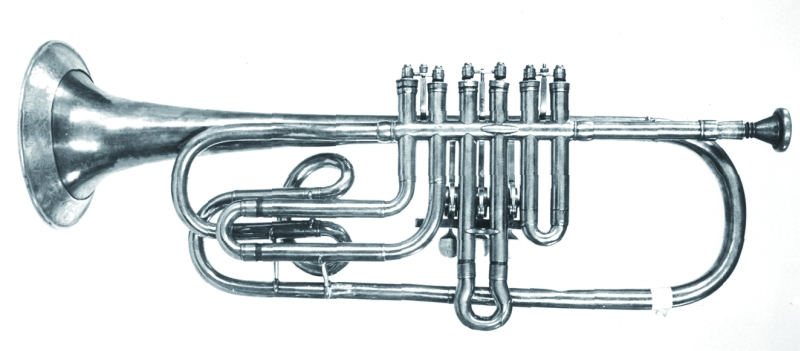
\includegraphics[width=\ratio\textwidth]{valve_trumpet}}{\ratio}
	\callout{-6 , 4}{ \1 }{-5.5 , 2}
	\callout{2 , 4}{ \2 }{2 , 2}
	\callout{6 , 4}{ \3 }{5 , 1}
	\callout{6, -4}{\4}{4, -2.5	}
	\callout{1.5, -4}{\5}{1.5, -2.5}
	\callout{-6, -4}{\6}{-4, -2}
	\helpgrid[black]
\end{annotate}
\caption{Callout with Texts}
\end{figure}
\blindtext
\pagebreak
%simulate longer texts with "pseudo translation"
\renewcommand{\1}{\tcbox[size=normal,on line, opacityframe=1]{****Bell****}}
\renewcommand{\2}{\tcbox[size=normal,on line, opacityframe=1]{****Valves****}}
\renewcommand{\3}{\tcbox[size=normal,on line, opacityframe=1]{****Mouthpiece****}}
\renewcommand{\4}{\tcbox[size=normal,on line, opacityframe=1]{****Valve slide****}}
\renewcommand{\5}{\tcbox[size=normal,on line, opacityframe=1]{****Valve slide****}}
\renewcommand{\6}{\tcbox[size=normal,on line, opacityframe=1]{****Hauptstimmung****}}
\blindtext
\begin{figure}[h]
	\begin{annotate}
		{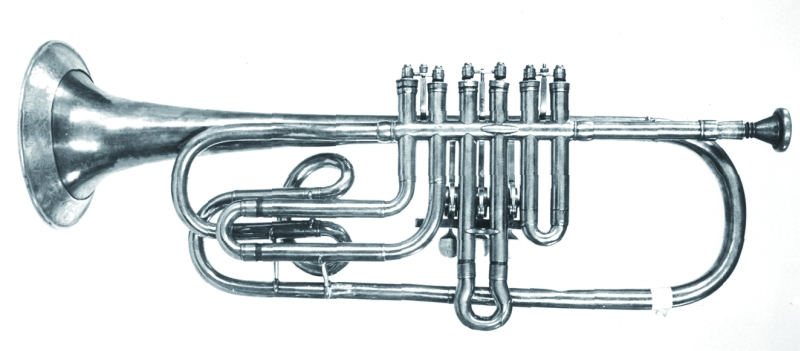
\includegraphics[width=\ratio\textwidth]{valve_trumpet}}{\ratio}
		\callout{-6 , 4}{ \1 }{-5.5 , 2}
		\callout{2 , 4}{ \2 }{2 , 2}
		\callout{6 , 4}{ \3 }{5 , 1}
		\callout{6, -4}{\4}{4, -2.5	}
		\callout{1.5, -4}{\5}{1.5, -2.5}
		\callout{-6, -4}{\6}{-4, -2}
		%\note{1, 2}{Text}
		%\arrow{2,3}{5,5}
		\helpgrid[black]
	\end{annotate}
	\caption{Callout mit ***Text***}
\end{figure}
\blindtext
\pagebreak
\renewcommand{\1}{\tcbox[size=small,on line, opacityframe=1]{Bell}}
\renewcommand{\2}{\tcbox[size=small,on line, opacityframe=1]{Valves}}
\renewcommand{\3}{\tcbox[size=small,on line, opacityframe=1]{Mouthpiece}}
\renewcommand{\4}{\tcbox[size=small,on line, opacityframe=1]{Valve slide}}
\renewcommand{\5}{\tcbox[size=small,on line, opacityframe=1]{Valve slide}}
\renewcommand{\6}{\tcbox[size=small,on line, opacityframe=1]{Hauptstimmung}}
\renewcommand{\ratio}{0.5}
\blindtext
\newline
\begin{minipage}{0.5\textwidth}
\blindtext
\end{minipage}
\begin{minipage}{\ratio\textwidth}
	\centering
	\begin{annotate}
		{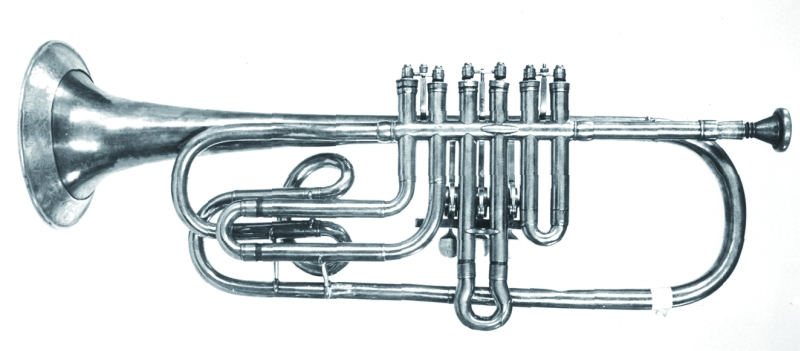
\includegraphics[width=\ratio\textwidth]{valve_trumpet}}{\ratio}
		\callout{-3 , 3}{ \1 }{-3 , 1.5}
		\callout{1 , 3}{ \2 }{1 , 1.5}
		\callout{3.5 , 3}{ \3 }{3.5 , 1}
		\callout{3, -3}{\4}{3, -1.5	}
		\callout{1, -3}{\5}{1, -1.5}
		\callout{-3, -3}{\6}{-2, -1.5}
		
	\end{annotate}
\end{minipage}
\blindtext

\pagebreak
%define callouts as numbers
\renewcommand{\1}{\tcbox[size=normal,on line, opacityframe=1]{1}}
\renewcommand{\2}{\tcbox[size=normal,on line, opacityframe=1]{2}}
\renewcommand{\3}{\tcbox[size=normal,on line, opacityframe=1]{3}}
\renewcommand{\4}{\tcbox[size=normal,on line, opacityframe=1]{4}}
\renewcommand{\5}{\tcbox[size=normal,on line, opacityframe=1]{5}}
\renewcommand{\6}{\tcbox[size=normal,on line, opacityframe=1]{6}}
\renewcommand{\ratio}{1}
\blindtext
\begin{figure}[h]
	
	\begin{annotate}
		{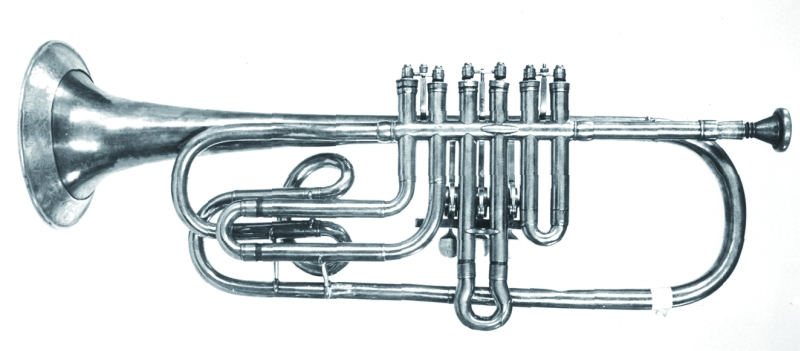
\includegraphics[width=\ratio\textwidth]{valve_trumpet}}{\ratio}
		\callout{-6 , 4}{ \1 }{-5.5 , 2}
		\callout{2 , 4}{ \2 }{2 , 2}
		\callout{6 , 4}{ \3 }{5 , 1}
		\callout{6, -4}{\4}{4, -2.5	}
		\callout{1.5, -4}{\5}{1.5, -2.5}
		\callout{-6, -4}{\6}{-4, -2}
		%\note{1, 2}{Text}
		%\arrow{2,3}{5,5}
		\helpgrid[black]
	\end{annotate}
	\caption{Callout with Numbers}
\end{figure}
\blindtext

\pagebreak
%small callout with legend table
\renewcommand{\1}{\tcbox[size=small,on line, opacityframe=1]{1}}
\renewcommand{\2}{\tcbox[size=small,on line, opacityframe=1]{2}}
\renewcommand{\3}{\tcbox[size=small,on line, opacityframe=1]{3}}
\renewcommand{\4}{\tcbox[size=small,on line, opacityframe=1]{4}}
\renewcommand{\5}{\tcbox[size=small,on line, opacityframe=1]{5}}
\renewcommand{\6}{\tcbox[size=small,on line, opacityframe=1]{6}}
\renewcommand{\ratio}{0.5}
\blindtext
\newline
\begin{minipage}{\ratio\textwidth}
	\centering
\begin{tabular}{ll}
	1 & Bell\\
	2 & Valves\\
	3 & Mouthpiece \\
	4 & Valve slide \\
	5 & Valve slide \\
	6 & Hauptstimmung \\
\end{tabular}
\end{minipage}
\begin{minipage}{\ratio\textwidth}
\centering
\begin{annotate}
	{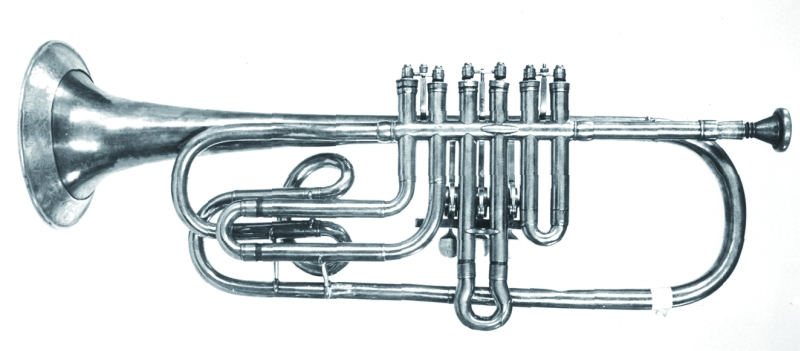
\includegraphics[width=\ratio\textwidth]{valve_trumpet}}{\ratio}
	\callout{-3 , 3}{ \1 }{-3 , 1.5}
	\callout{1 , 3}{ \2 }{1 , 1.5}
	\callout{3.5 , 3}{ \3 }{3.5 , 1}
	\callout{3, -3}{\4}{3, -1.5	}
	\callout{1, -3}{\5}{1, -1.5}
	\callout{-3, -3}{\6}{-2, -1.5}

\end{annotate}
\end{minipage}
\blindtext
\pagebreak
\renewcommand{\ratio}{0.5}
\blindtext
\newline
\begin{minipage}{0.5\textwidth}
	\blindtext
\end{minipage}
\begin{minipage}{\ratio\textwidth}
	\centering
	\begin{annotate}
		{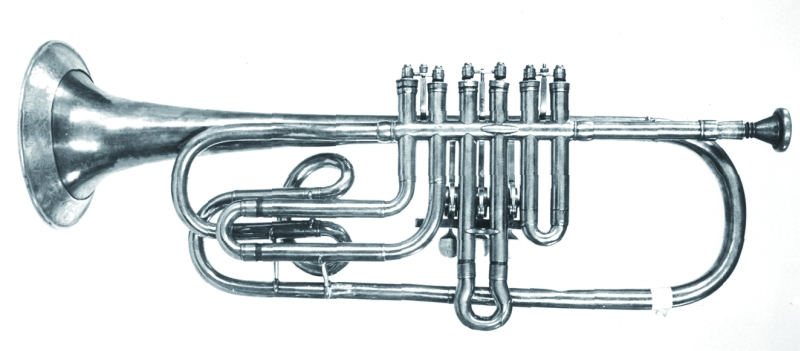
\includegraphics[width=\ratio\textwidth]{valve_trumpet}}{\ratio}
		\draw[ thick,\arcol ](-4 ,-1) rectangle (-3 ,1.5);
		\helpgrid[black]
	\end{annotate}
\end{minipage}
\blindtext

\end{document}


